% Owner: B -- measured CIT contribution only.
\paragraph{Citation network (CIT).}
In 2020, annual and cumulative graphs on the same 19,150 born nodes contain
1,450 and 73,269 citations. Mean total degree is 0.151 versus 7.652, weak
largest-component fraction 0.052 versus 0.641, and cumulative weak clustering
0.124. Annual clustering is identically zero: strict older-target citations make
each annual snapshot bipartite. This is a consequence of the representation,
not independent evidence for temporal correlations. Over 1-, 2-, 5- and 10-year
windows, relative ranges average 1.798 for density/degree, 2.361 for clustering
and 1.114 for largest-component fraction.
\textbf{CIT verdict on H1:} window choice changes structural descriptions;
some differences are definitional. The node denominator and year convention
must accompany every comparison.

\begin{figure*}[t]
\centering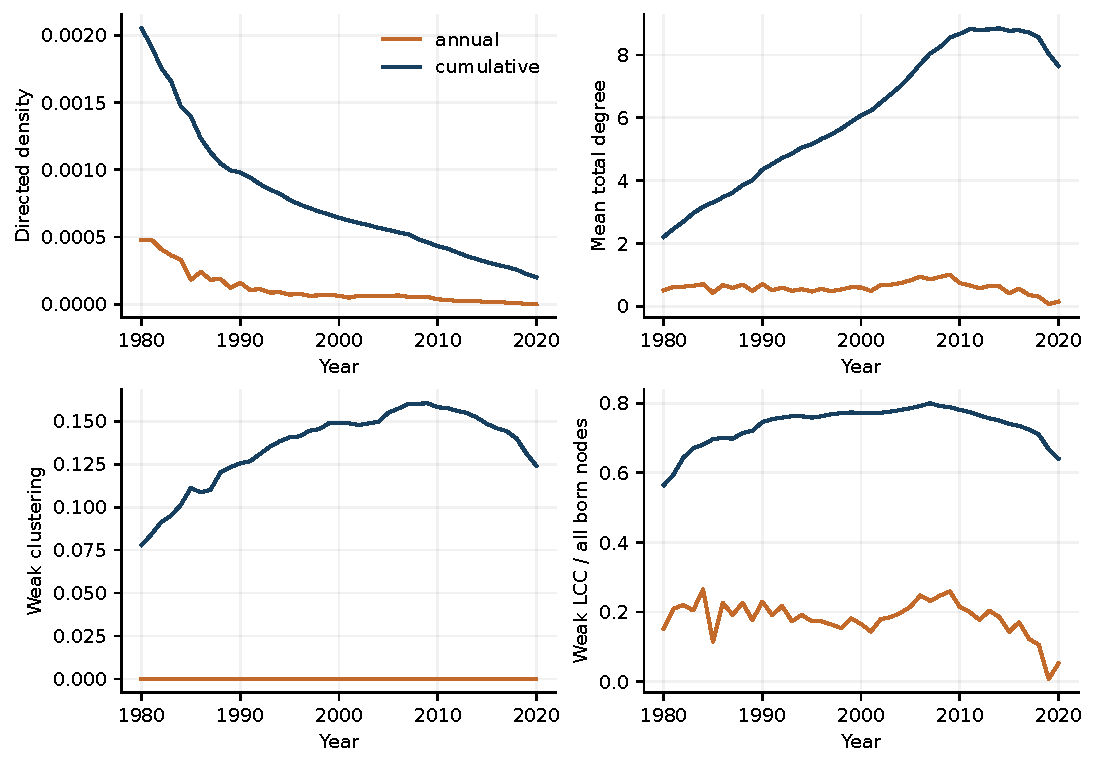
\includegraphics[width=.95\textwidth]{b_aggregation.pdf}
\caption{Measured CIT annual and cumulative structure, including born isolates.
The annual zero clustering is imposed by strict publication-year ordering.}
\label{fig:b-aggregation}
\end{figure*}

\paragraph{Window interpretation.}
\Cref{fig:b-window} shows that longer windows connect a larger fraction of born
papers and admit cross-year triangles. These effects require a sequence of
snapshots; one final aggregate cannot reveal when connectivity appears.
The relative range is a window-sensitivity statistic, not a significance test
against a temporal null, and identical density/degree sensitivity follows from
the common denominator.

\begin{figure*}[t]
\centering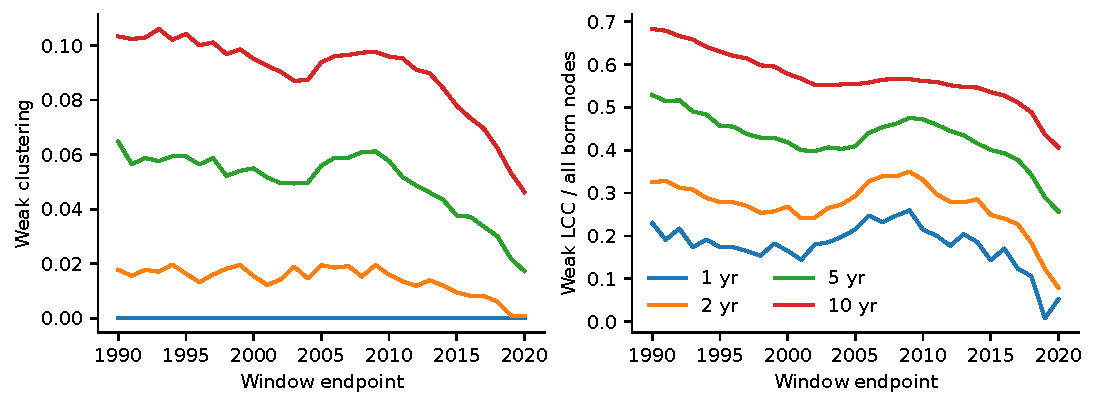
\includegraphics[width=.95\textwidth]{b_window_sensitivity.pdf}
\caption{Measured CIT trailing-window clustering and connectivity for 1, 2, 5
and 10 years. Born isolates are included at every endpoint.}
\label{fig:b-window}
\end{figure*}
